
\section{Example Using Two Tetrahedra with Georeferenced Coordinate System Mesh}
\label{sec:examples:twotet4-geoproj}

PyLith features discussed in this example:
\begin{itemize}
\item Quasi-static solution
\item Mesh ASCII format
\item Dirichlet boundary conditions
\item Kinematic fault interface conditions
\item Linearly elastic isotropic material
\item VTK output
\item Linear tetrahedral cells
\item SimpleDB spatial database with geographic coordinates
\item SCEC CVM-H spatial database
\item ZeroDispDB spatial database
\end{itemize}
All of the files necessary to run the examples are contained in the
directory \filename{examples/twocells/twotet4-geoproj.}


\subsection{Overview}

This example is virtually identical to the other example using two
linear tetrahedra (See Section \vref{sec:example:twotet4}). The
primary difference is in how the material properties are assigned.
For this example, the physical properties come from the SCEC CVM-H
database (described in Section \vref{sec:SCEC:CVM-H}). Using the SCEC
CVM-H database is straightforward, requiring only a few modifications
to \filename{pylithapp.cfg}. Because the SCEC CVM-H database uses
geographic coordinates, we must also use geographic coordinates in the
PyLith mesh ASCII file and other spatial databases. Note that all of
these geographic coordinate systems do not need to be the same. PyLith
will automatically transform from one geographic coordinate system to
another using the spatialdata package. The spatial databases should
all use a georeferenced Cartesian coordinate system, such as a
geographic projection to insure interpolation is performed
properly. Since all aspects of this problem other than the material
database and the coordinate system are identical to the examples in
Section \vref{sec:example:twotet4}, we only describe the kinematic
fault problem in this example.


\subsection{Mesh Description}

The mesh consists of two tetrahedra forming a pyramid shape (Figure
\vref{fig:twotet4-geoproj-mesh}). The mesh geometry and topology are
described in the file \filename{twotet4.mesh}, which is in PyLith mesh
ASCII format. If you compare this mesh against the one used in \vref{sec:example:twotet4},
you will notice that, although the mesh topology is the same, the
vertex coordinates are significantly different. We use zone 11 UTM
coordinates with the NAD27 datum for the mesh. Although we used the
same coordinate system as the SCEC CVM-H, we could have also used
any other geographic projection supported by spatialdata and Proj.4.
See Appendix \vref{sec:format:SimpleIOAscii} for other examples
of using geographic coordinates. 

\begin{figure}
  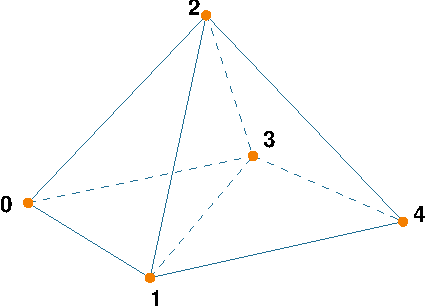
\includegraphics{examples/figs/twotet4-mesh}
  \caption{Mesh composed of two linear tetrahedral cells in a
    georeferenced coordinate system used for the example problems.}
  \label{fig:twotet4-geoproj-mesh}
\end{figure}

\subsection{Additional Common Information}

This problem has some unique aspects compared to the other examples.
First, all of the other examples use a Cartesian coordinate system,
while this one uses a geographic coordinate system. In addition to
using different vertex coordinates, we also define the coordinate
system for the mesh in \filename{pylithapp.cfg}:
\begin{cfg}
<h>pylithapp.mesh_generator.importer]</h>
<f>coordsys</f> = spatialdata.geocoords.CSGeoProj
<p>filename</p> = twotet4.mesh
<p>coordsys.space_dim</p> = 3

<h>[pylithapp.mesh_generator.importer.coordsys]</h>
<p>datum_horiz</p> = NAD27
<p>datum_vert</p> = mean sea level
<p>ellipsoid</p> = clrk66

<h>[pylithapp.mesh\_generator.importer.coordsys.projector]</h>
<p>projection</p> = utm
<p>proj-options</p> = +zone=11
\end{cfg}
At the top level, we define the type of coordinate system, give the
file describing the mesh, and give the number of spatial dimensions
for the coordinate system. We then provide the horizontal datum and
vertical datum for the coordinate system, along with the ellipsoid
to be used. Finally, we specify a UTM projection, and specify zone
11 as the zone to be used.

In addition to the usual material information, we must specify that
we want to use the \object{SCECCVMH} database implementation:
\begin{cfg}
<h>[pylithapp.timedependent.materials.material]</h>
<f>db</f> = spatialdata.spatialdb.SCECCVMH
<p>db.data_dir</p> = /home/john/data/sceccvm-h/vx53/bin
\end{cfg}
The first \facility{db} option defines \object{SCECCVMH} as the
spatial database to be used. The next line defines the location of the
\filename{vx53} data files, and must be changed to the location
specified by the user when the package is installed. The package may
be obtained from Harvard's Structural Geology and Tectonics
\url{structure.harvard.edu/cvm-h}.

The final difference with the other examples is in the description of
the spatial databases. They must also use geographic coordinates.
Examining \filename{dislocation\_slip.spatialdb}, we find:
\begin{SimpleIOAscii}
// We are specifying the data in a projected geographic coordinate system.
cs-data = geo-projected {
  to-meters = 1.0
  ellipsoid = clrk66
  datum-horiz = NAD27
  datum-vert = mean sea level
  projector = projection {
    projection = utm
    units = m
    proj-options = +zone=11
  }
}
\end{SimpleIOAscii}

\subsection{Kinematic Fault Slip Example}

This example problem is a left-lateral fault slip applied between
the two tetrahedral cells using kinematic cohesive cells. Note that
we vary the amount of fault slip for each vertex with this example,
as described in 
\filename{dislocation\_slip.spatialdb}. The vertices away from the fault
are held fixed in the x, y, and z directions. Parameter settings that
override or augment those in \filename{pylithapp.cfg} are contained
in the file \filename{dislocation.cfg}.

Recall that we condition problems with the kinematic fault interface
using the material properties. Since the material properties are being
defined using the SCEC CVM-H database, this same database should be
used as the material database for the faults. This also applies to
the AbsorbingDampers boundary condition.

The files containing common information (\filename{twotet4.mesh}, \filename{pylithapp.cfg})
along with the problem-specific files (\filename{dislocation.cfg, dislocation\_slip.spatialdb,
dislocation\_sliptime.spatialdb}) provide a complete description of
the problem, and we can then run this example by typing
\begin{shell}
$$ pylith dislocation.cfg
\end{shell}
If the problem ran correctly, you should be able to generate a figure
such as Figure \vref{fig:twotet4-geoproj-disloc}, which was generated
using ParaView.

\begin{figure}
  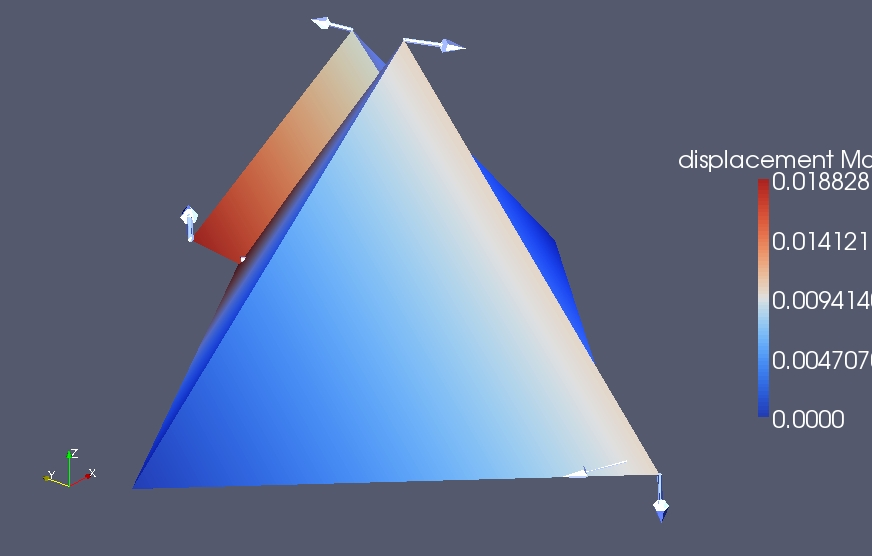
\includegraphics[scale=0.33]{examples/figs/twotet4-geoproj-dislocation}
  \caption{Color contours and vectors of displacement for the kinematic fault
    example using a mesh composed of two linear tetrahedral cells in a
    georeferenced coordinate system.}
  \label{fig:twotet4-geoproj-disloc}
\end{figure}


% End of file

